\documentclass{protokol}
\leftheader{Vláknová optika}
\centerheader{Praktikum III}
\rightheader{Tomáš Derner}

\begin{document}

  \section*{Úkol}

    \begin{enumerate}
      \item Navažte laserový svazek do vlákna a seřiďte jednotlivé moduly tak, abyste dosáhli maximálního výkonu na výstupu z vlákna.
      \item Změřte numerickou aperturu vlákna, zpracujte graficky.
      \item Změřte dobu průchodu světla vláknem, určete rychlost světla ve vlákně.
      \item Změřte světelné charakteristiky laseru pro tři různé teploty laserového modulu, sledujte vliv teploty na prahový proud.
    \end{enumerate}

  \section*{Teorie}

    Optické vlákno se skládá z jádra a pláště, přičemž index lomu jádra je vyšší než index lomu pláště. Na rozhraní těchto dvou tedy dochází k totálnímu odrazu.
    V tomto praktiku pracujeme s aparaturou popsanou ve studijním textu \cite{pokyny}.

    Teoretickou numerickou aperturu spočteme pomocí vztahu 
    \begin{equation} \label{eq:teor_apertura}
      A_{teor} = \sqrt{n_j^2 - n_p^2},
    \end{equation}
    kde $n_j$ a $n_p$ jsou indexy lomu jádra resp. pláště. V tomto praktiku jsou tyto hodnoty
    $$ n_j = \num{1.465}, $$
    $$ n_p = \num{1.462}. $$

    Experimentálně lze aperturu získat měřením výstupního výkonu v různých úhlech. Z naměřené závislosti určíme úhly $\Theta$ od maximálního bodu průběhu, při kterých klesne výkon na $\frac{1}{e^2}$ maximální hodnoty. Aperturu pak spočteme jako 
    \begin{equation}
      A = sin \Theta.
    \end{equation}
    Protože však maximální hodnota průběhu nemusí nastat právě při nulovém úhlu aparatury $\varphi$, počítáme úhel $\Theta$ právě od maxima průběhu.

    Dobu průchodu světla vláknem a potažmo rychlost světla získáme odečtením doby $T_1$, za kterou světelný signál projde aparaturou bez zařazeného optického vlákna, od doby $T_2$ průchodu světla aparaturou s vláknem,
    \begin{equation}
      \tau = T_2 - T_1.
    \end{equation}
    Z toho pak získáme rychlost světla v prostředí s indexem lomu $n_j$ podle vztahu 
    \begin{equation}
      v = \frac{l}{\tau},
    \end{equation}
    kde $l$ je délka vlákna.

    Teoretickou hodnotu rychlosti světla vláknem určíme ze vztahu
    \begin{equation} \label{eq:v_teor}
      v_{teor} = \frac{c}{n_j},  
    \end{equation} 
    kde $c \doteq \SI{3e8}{\metre\per\second}$ je rychlost světla ve vakuu.

  \section*{Výsledky}

    \subsection*{Úkol 2}

      S pomocí osciloskopu jsme proměřili úhlové rozložení výkonu světla prošlého vláknem, výsledné hodnoty byly fitovány gaussovským rozložením, jak je znázorněno v grafu \ref{fig:apertura}. Zároveň je zde zobrazena hodnota $\frac{1}{e^2}$ maximální hodnoty průběhu.

      \begin{figure}[H]
        \centering
        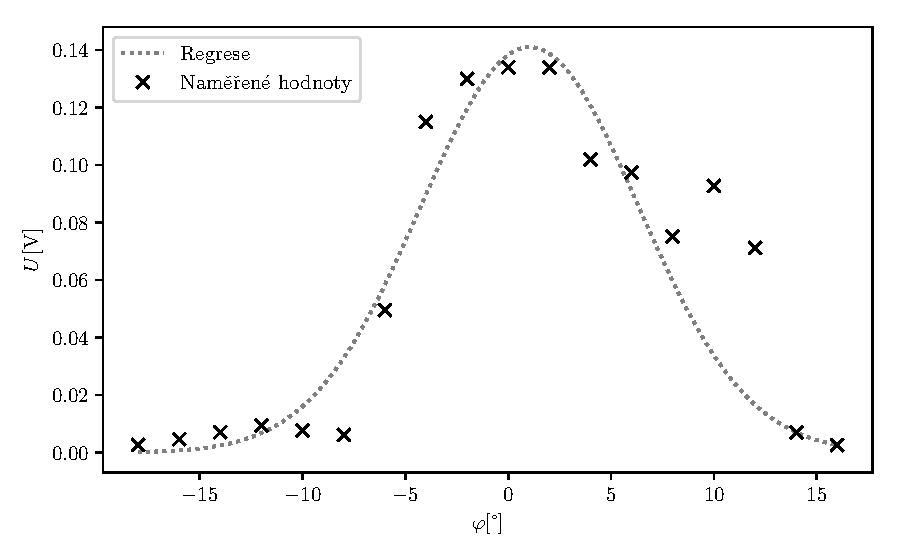
\includegraphics[]{apertura}
        \caption{Závislost napětí na fotodiodě na úhlu ramena aparatury}
        \label{fig:apertura}
      \end{figure}

      Z grafu odečteme úhlovou vzdálenost $\Theta$ průsečíku tečkovaně vyznačené hranice s čárkovaně značeným průběhem závislosti od polohy středu průběhu
      $$ \Theta = \SI{10.6 \pm 1}{\degree}. $$
      Z tohoto určíme hodnotu numerické apertury
      $$ A = \num{0.18 \pm 0.02}. $$

      Pomocí vztahu \eqref{eq:teor_apertura} spočteme teoretickou numerickou aperturu
      $$ A_{teor} \doteq \num{0.094}. $$ 
 
    \subsection*{Úkol 3}

      Pomocí osciloskopu byly naměřeny doby průchodu světla aparaturou bez a s optickým vláknem
      $$ T_1 = \SI{0.10 \pm 0.05 e-6}{\second}, $$
      $$ T_2 = \SI{5.44 \pm 0.05 e-6}{\second}. $$

      Doba průchodu světla vláknem je pak 
      $$ \tau = \SI{5.34 \pm 0.07 e-6}{\second}. $$

      Pro délku vlákna 
      $$ l = \SI{1212 \pm 20}{m} $$
      určíme rychlost světla ve vláknu 
      $$ v = \SI{227 \pm 5 e6}{\metre\per\second}. $$

      Teoretickou hodnotu této veličiny určíme ze vztahu \eqref{eq:v_teor},
      $$ v_{teor} \doteq \SI{204 e6}{\metre\per\second}. $$

    \subsection*{Úkol 4}

      Pomocí osciloskopu byly naměřeny světelné charakteristiky laseru pro teploty $10, 20$ a $\SI{30}{\celsius}$. Tyto charakteristiky jsou zobrazeny v grafu \ref{fig:teploty}. Ačkoli zobrazením všech dat do jednoho grafu poněkud utrpěla přehlednost bodů jednotlivých naměřených hodnot, toto rozhodnutí bylo učiněno s cílem znázornit vzájemnou polohu regresních přímek.

      \begin{figure}[H]
        \centering
        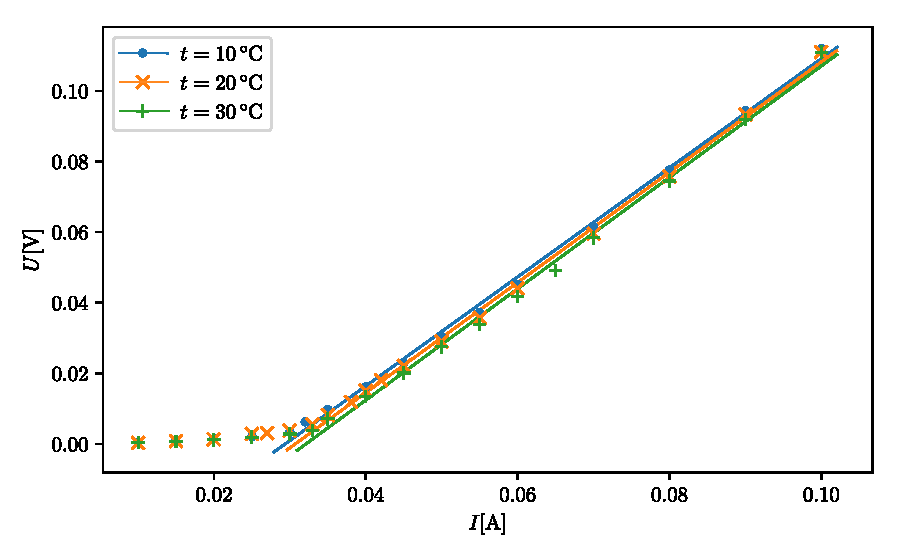
\includegraphics[]{teploty}
        \caption{Světelné charakteristiky laseru při různých teplotách}
        \label{fig:teploty}
      \end{figure}

      Prahové proudy byly určeny jako průsečíky regresních přímek s osou X.
      $$ I_{\SI{10}{\celsius}} = \SI{0.029 \pm 0.001}{mA}, $$
      $$ I_{\SI{20}{\celsius}} = \SI{0.030 \pm 0.001}{mA}, $$
      $$ I_{\SI{30}{\celsius}} = \SI{0.032 \pm 0.001}{mA}.  $$

  \section*{Diskuse}

    Srovnáním spočtených hodnot veličin s teoretickými předpověďmi je zřejmé, že toto měření bylo poměrně nepřesné. Numerická apertura experimentálně vyšla dvojnásobná oproti teoretické hodnotě s nejvyšší pravděpodobností kvůli nedokonalému zakončení optického vlákna, které bylo mikroskopem pozorováno již v průběhu měření. Podle komentáře asistenta praktika však nebylo vůbec jasné, zda by seříznutí optického vlákna situaci vyřešilo či naopak značně zkomplikovalo, proto bylo od tohoto kroku upuštěno.

    Velká odchylka hodnoty rychlosti světla ve vláknu oproti teorii byla do určité míry očekávaná, podle informací asistenta praktika je totiž hodnota délky vlákna či hodnota jeho indexu lomu v praktiku uvedena značně nepřesně, odhlédneme-li od přidané chyby způsobené postupným krácením vlákna (tato skutečnost je reflektována zvolením vysoké chyby u hodnoty délky vlákna).

  \section*{Závěr}

    Byl úspěšně navázán laserový svazek do optického vlákna.

    Byla změřena numerická apertura 
    $$ A = \num{0.18 \pm 0.02}. $$

    Byla určena doba průchodu světla vláknem a rychlost světla ve vlákně
    $$ \tau = \SI{5.34 \pm 0.07 e-6}{\second}, $$
    $$ v = \SI{227 \pm 5 e6}{\metre\per\second}. $$

    Byly změřeny světelné charakteristiky laseru pro tři různé teploty laserového modulu a určeny prahové proudy
    $$ I_{\SI{10}{\celsius}} = \SI{0.029 \pm 0.001}{mA}, $$
    $$ I_{\SI{20}{\celsius}} = \SI{0.030 \pm 0.001}{mA}, $$
    $$ I_{\SI{30}{\celsius}} = \SI{0.032 \pm 0.001}{mA}.  $$
      
  \begin{thebibliography}{}
 
    \bibitem{pokyny}
    Pokyny k měření ``Vlnová optika'', dostupné z\\ \url{http://physics.mff.cuni.cz/vyuka/zfp/_media/zadani/pokyny/mereni_326.pdf}, 5.\,4.\,2018
   
  \end{thebibliography}

\end{document} 